\documentclass[12pt,a4paper]{article}
\usepackage[UTF8]{ctex}     %先引入ctex
\usepackage[utf8]{inputenc} %再引入inputenc
\usepackage{graphicx}
\usepackage{geometry}
\usepackage{xcolor}
% \usepackage{lazylatex}
\usepackage{amsmath}
\usepackage{enumerate}
\usepackage{caption}
\usepackage{listings}
\captionsetup[lstlisting]{labelfont=bf,justification=justified}

\usepackage{tikz}
\usepackage{appendix}

\graphicspath{{img/}}
% 边距
\geometry{left=2.0cm,right=2.0cm,top=2.0cm,bottom=3.0cm}
% 大题
\newenvironment{problems}{\begin{list}{}{\renewcommand{\makelabel}[1]{\textbf{##1}\hfil}}}{\end{list}}
% 小题
\newenvironment{steps}{\begin{list}{}{\renewcommand{\makelabel}[1]{##1.\hfil}}}{\end{list}}
% 答
\providecommand{\ans}{\textbf{答}:~}
% 解
\providecommand{\sol}{\textbf{解}.~}

\usepackage[colorlinks,linkcolor=blue]{hyperref}
\usepackage{bookmark}
\providecommand{\code}[2]{\lstinputlisting[language=#2,caption=\href{run:#1}{\ttfamily #1}]{#1}}
\providecommand{\img}[1]{\includegraphics[width=0.88\textwidth]{#1}}

% listings
\definecolor{grey}{rgb}{0.8,0.8,0.8}
\definecolor{darkgreen}{rgb}{0,0.3,0}
\definecolor{darkblue}{rgb}{0,0,0.3}
\lstset{%
    % numbers=left, %行号
    % numberstyle=\tiny\color{grey},
    showstringspaces=false,
    showspaces=false,%
    tabsize=4,%
    frame=shadowbox,%
    basicstyle={\ttfamily\scriptsize},%
    keywordstyle=\color{blue!80!black}\bfseries,%
    identifierstyle=,%
    commentstyle=\color{green!50!blue}\itshape,%
    stringstyle=\color{green!50!black},%
    rulesepcolor=\color{gray!20!white},
    breaklines,
    columns=flexible,
    extendedchars=false,
    %mathescape=true,
}

\begin{document}
\title{\normalsize \underline{操作系统(D)}\\\LARGE 项目 4}
\author{李子龙 518070910095}
\date{\today}
\maketitle

\textbf{调度算法}

\begin{problems}
    \item[一] \textbf{C 语言实现版本}
    \begin{steps}
        \item[1] FCFS
        
        \lstinputlisting[language=c,caption=\href{run:src/posix/schedule_fcfs.c}{\ttfamily src/posix/schedule\_fcfs.c}]{src/posix/schedule_fcfs.c}

        将输入的任务按照先后次序形成链表,注意第一个任务插入的时候特别进行了处理,之后按照给定的链表方法使用地址输入需要被替代位置的元素,之后顺移。遍历结果如下图所示:
        
        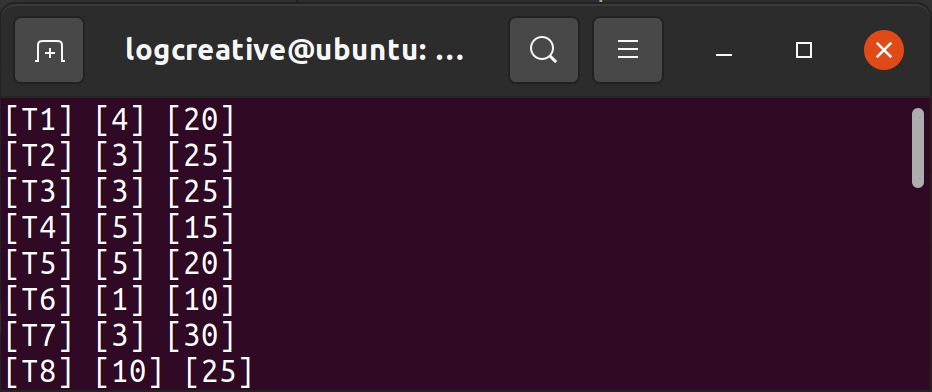
\includegraphics[width=0.6\textwidth]{traverse.png}

        之后按照 FCFS 的规则遍历该链表运行即可,运行完成后就会把链表上对应的元素删除。

        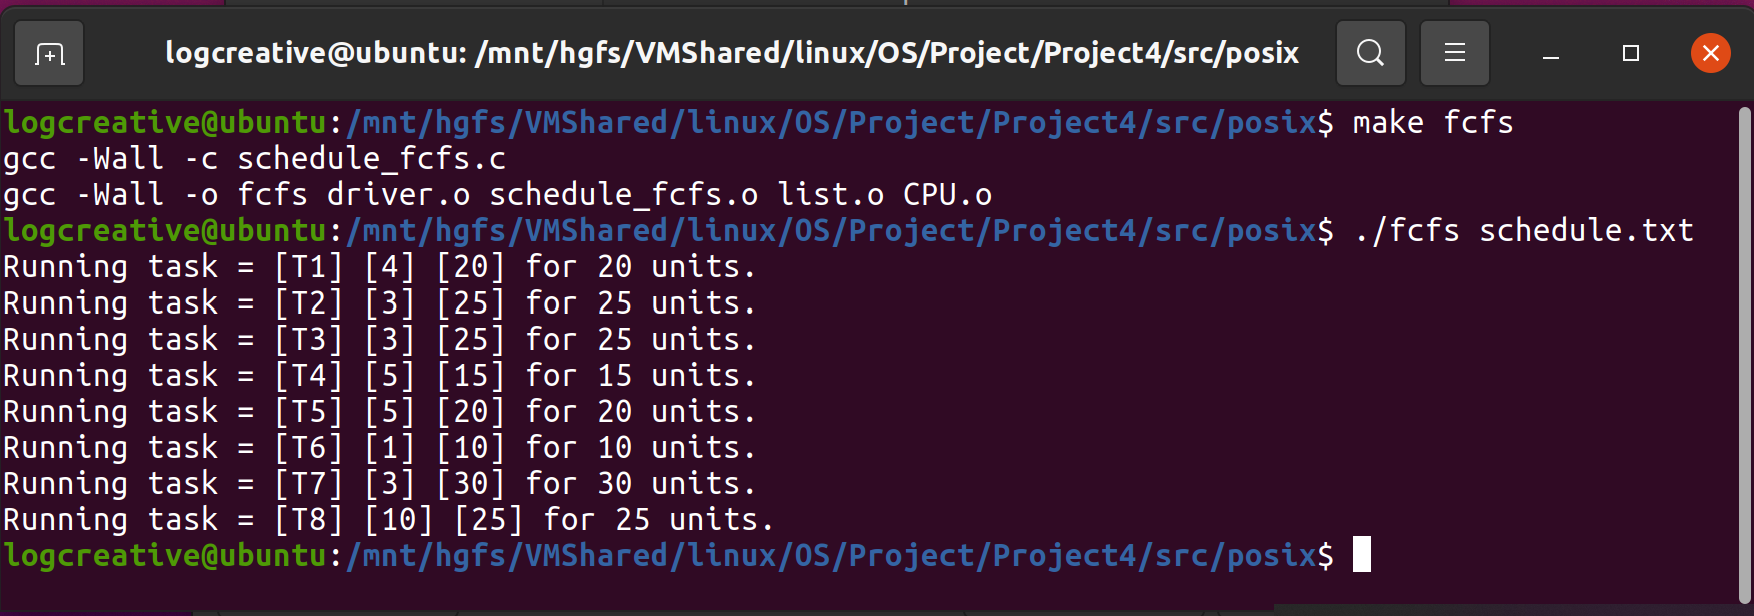
\includegraphics[width=0.8\textwidth]{fcfs.png}
        
        \item[2] SJF
        
        \lstinputlisting[language=c,caption=\href{run:src/posix/schedule_sjf.c}{\ttfamily src/posix/schedule\_sjf.c}]{src/posix/schedule_sjf.c}

        SJF 算法要求首先处理运行时间短的任务。这里采用了调度时寻找时间最短任务方法。每次对链表进行最小值搜索,存入 \verb"minNode" 中,使用小于号即可保证取的是同最小值的最先值。

        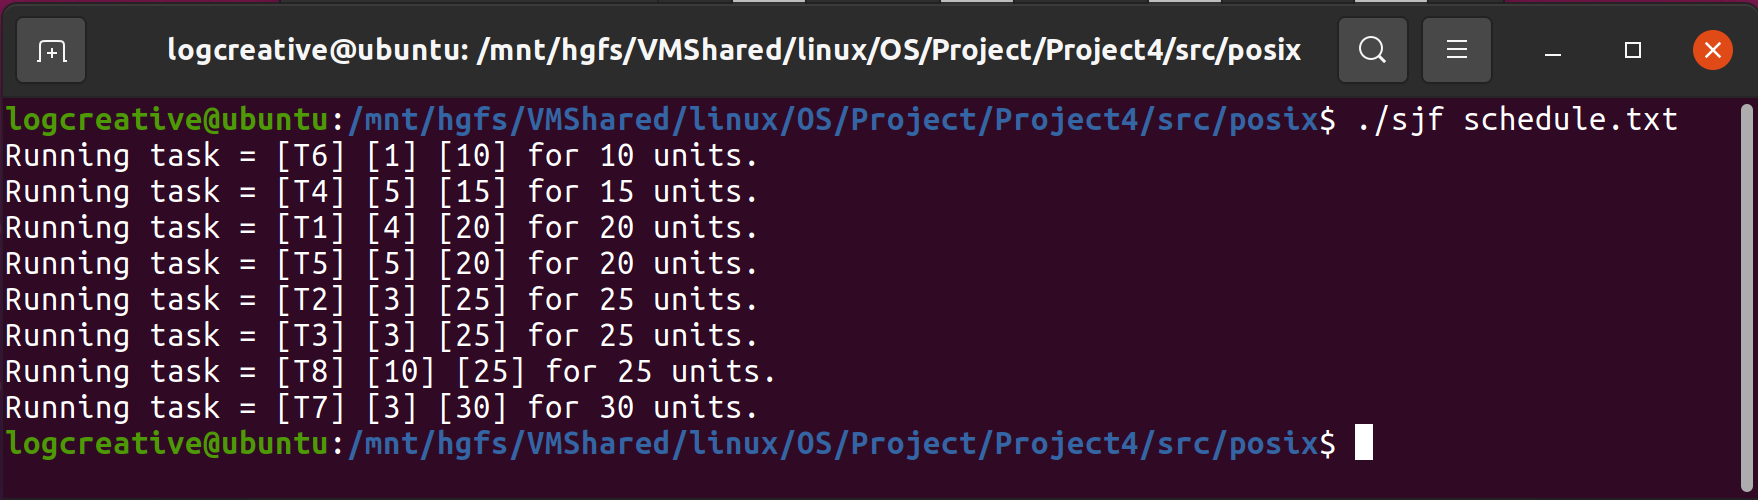
\includegraphics[width=0.88\textwidth]{sjf.png}

        \item[3] RR
        
        \lstinputlisting[language=c,caption=\href{run:src/posix/schedule_rr.c}{\ttfamily src/posix/schedule\_rr.c}]{src/posix/schedule_rr.c}

        轮转调度使用 FCFS 按照顺序让每一个任务运行一个时间量 \verb"QUANTUM" 的时间,一个未运行结束的程序会被插入到列表的最后。使用一个 \verb"pivot" 的指针追踪正在进行的任务。

        该算法在标准集和特集上的运行情况分别如下:

        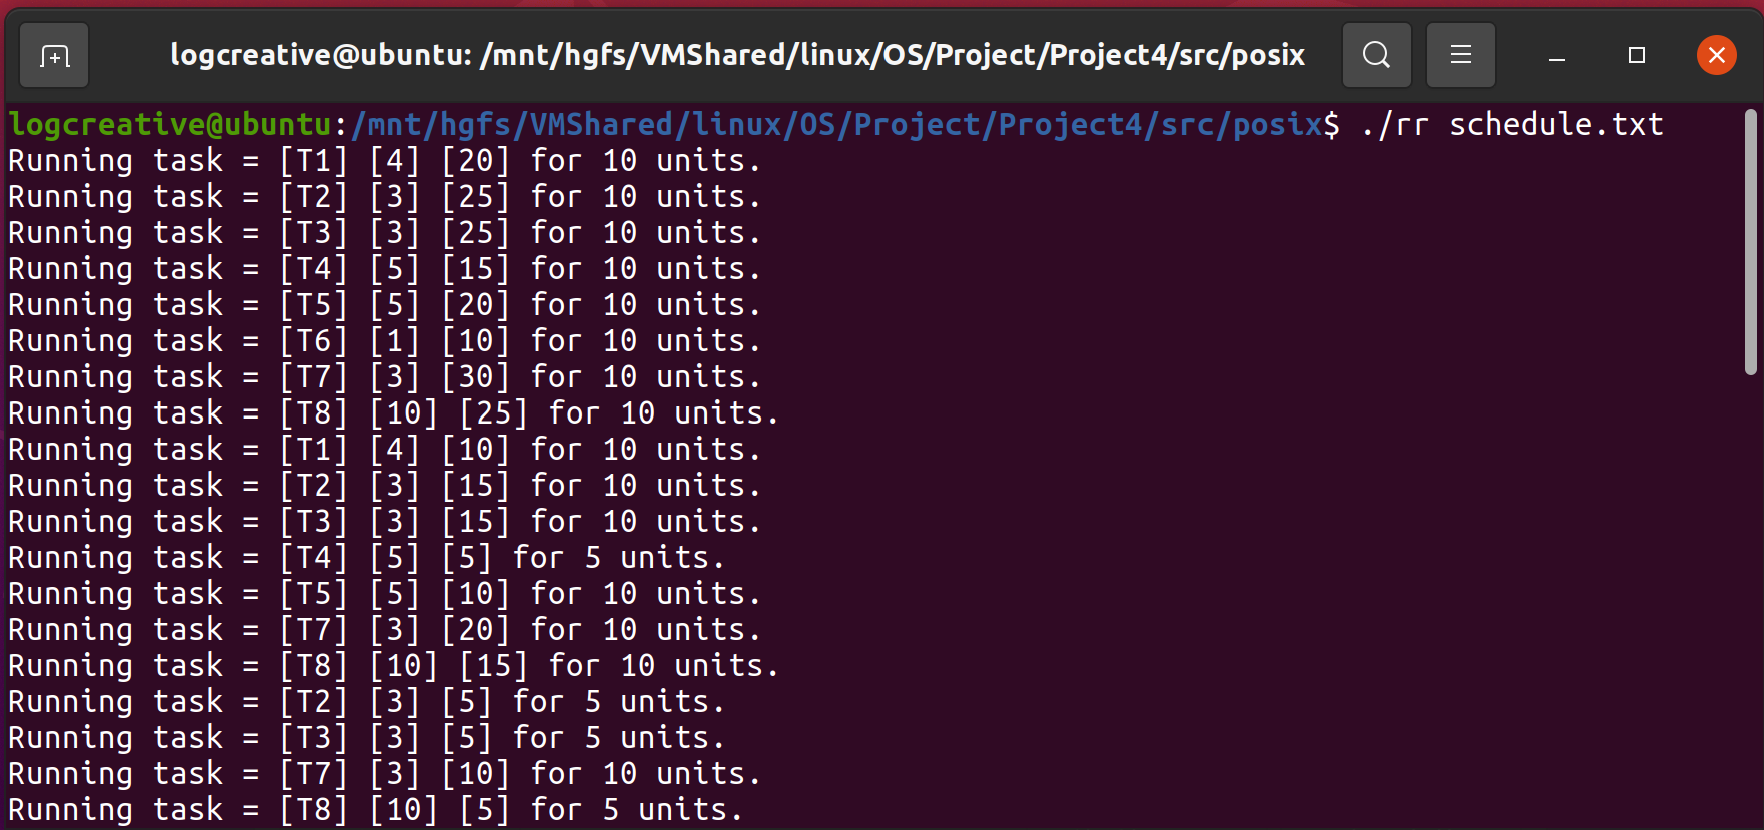
\includegraphics[width=0.8\textwidth]{rr1.png}

        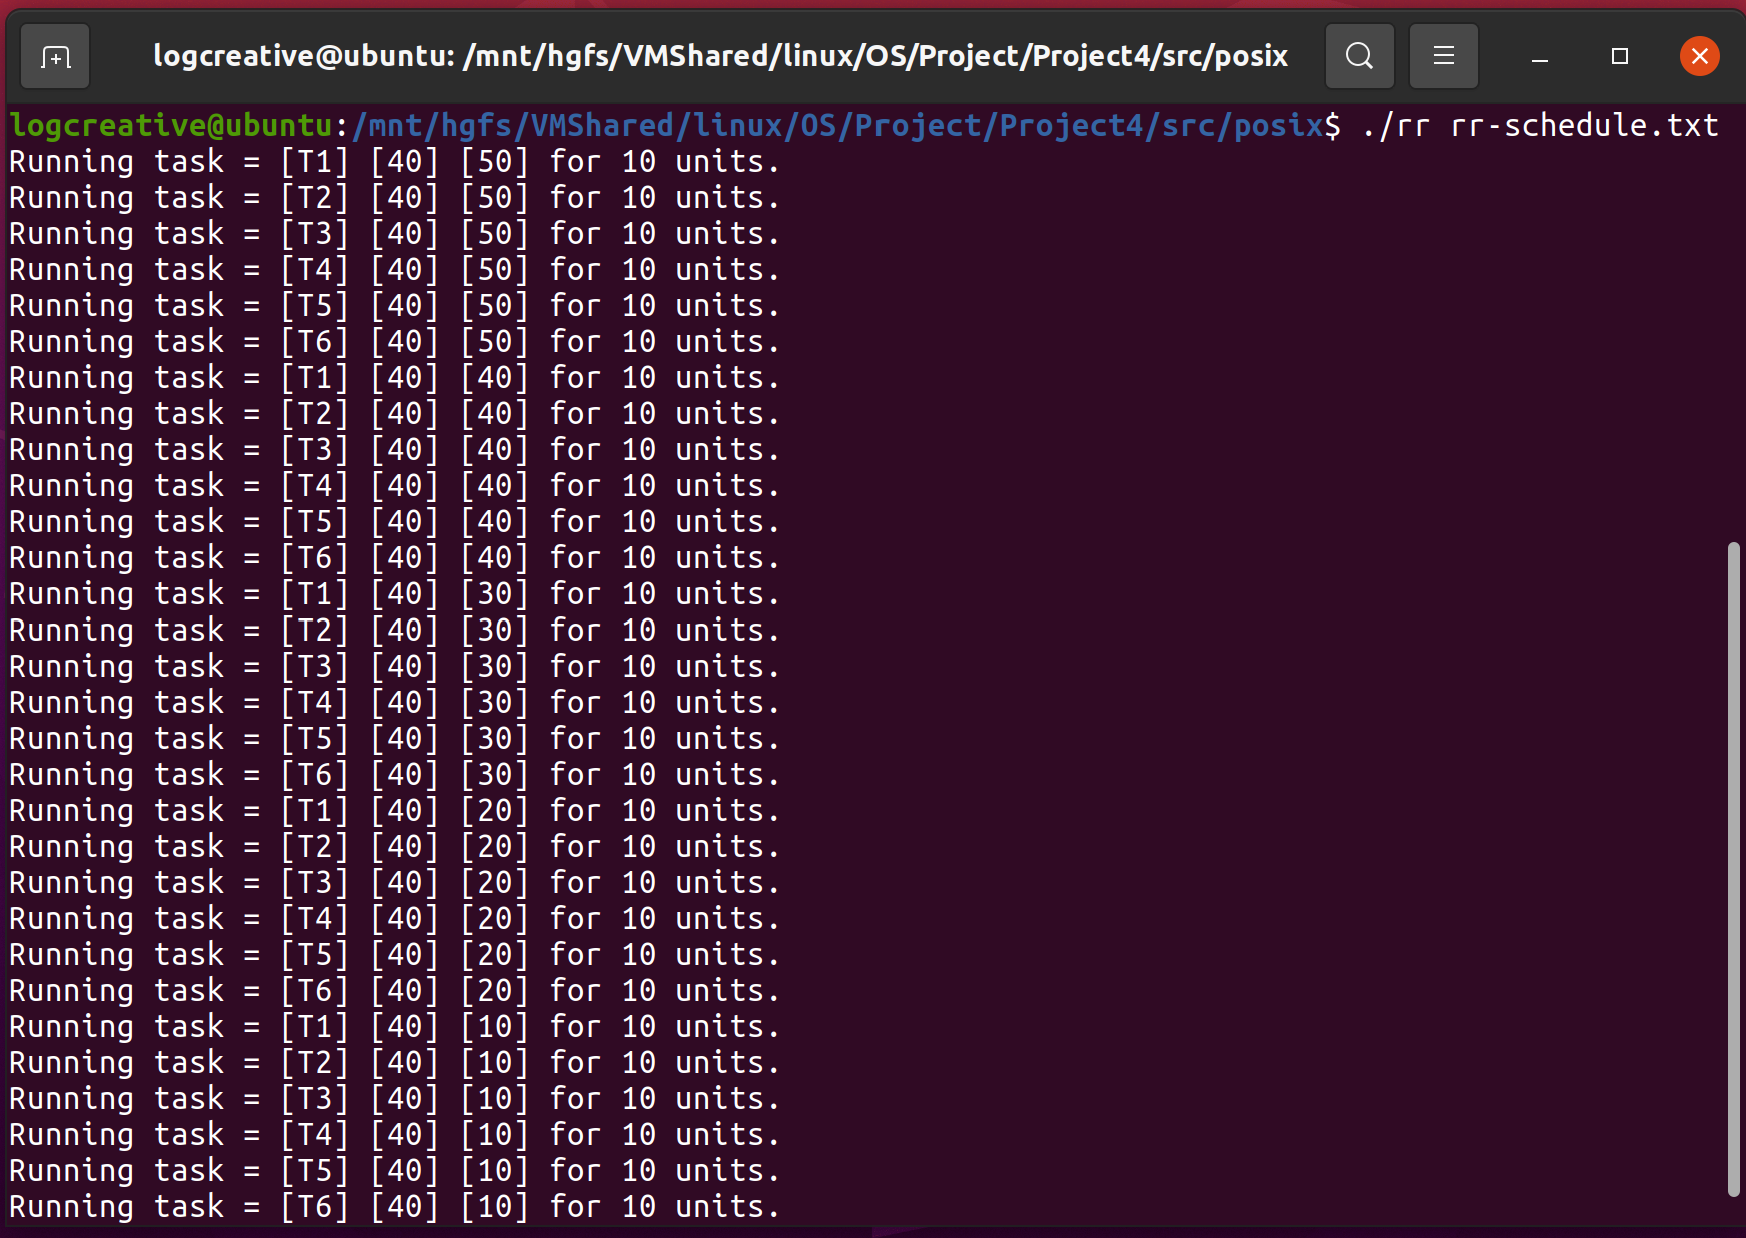
\includegraphics[width=0.8\textwidth]{rr2.png}

        \item[4] 优先级调度
        
        \lstinputlisting[language=c,caption=\href{run:src/posix/schedule_priority.c}{\ttfamily src/posix/schedule\_priority.c}]{src/posix/schedule_priority.c}

        类似于 SJF,只不过是比较的任务中优先级的最大值,同优先级取最先进行的。该算法在标准集与特集上的运行结果分别如下:

        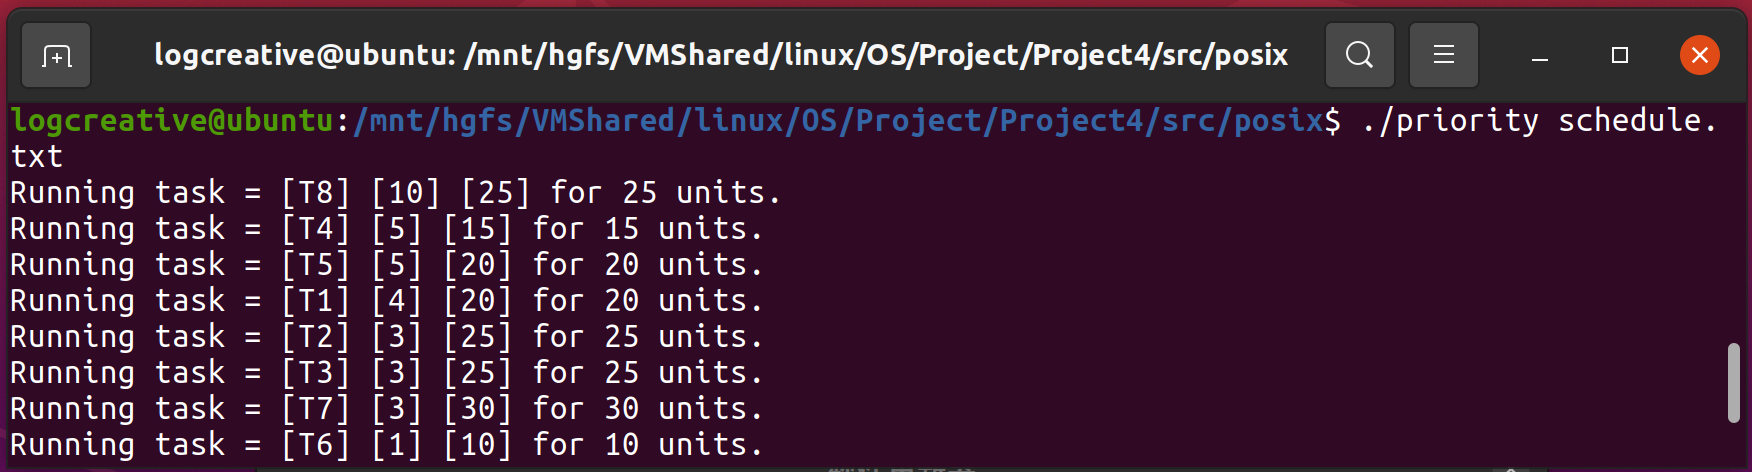
\includegraphics[width=0.8\textwidth]{pri1.png}

        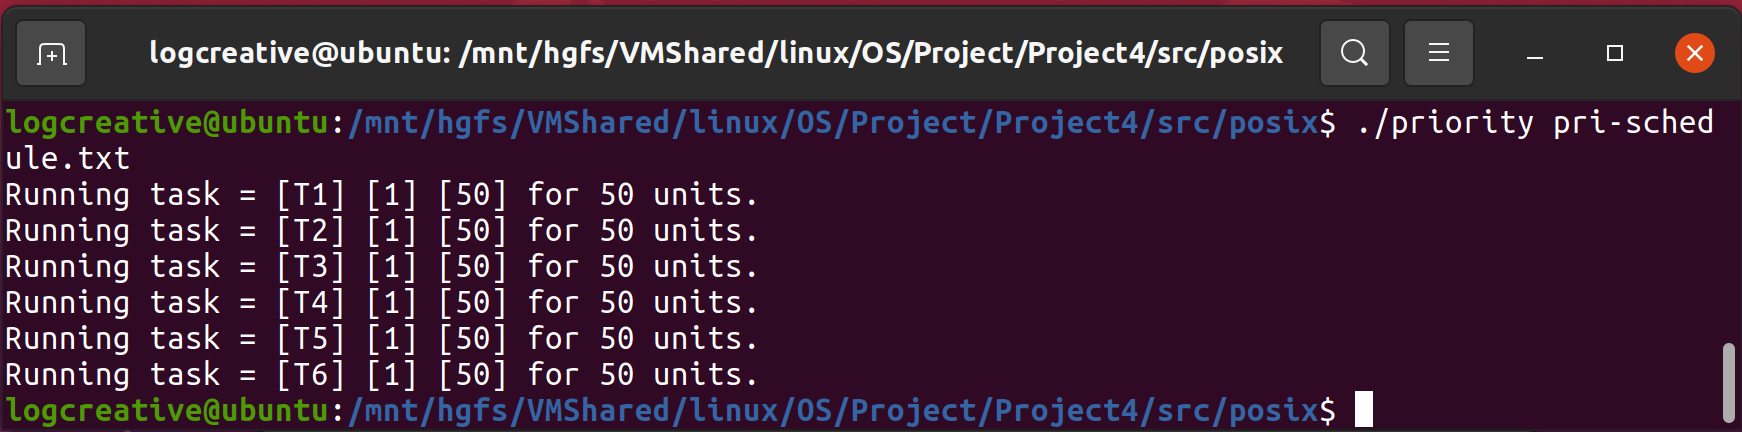
\includegraphics[width=0.8\textwidth]{pri2.png}
        
        \item[5] 优先级--轮转调度
        
        \lstinputlisting[language=c,caption=\href{run:src/posix/schedule_priority_rr.c}{\ttfamily src/posix/schedule\_priority\_rr.c}]{src/posix/schedule_priority_rr.c}

        优先级--轮转调度需要同时考虑两者,则在开始的加入 \verb"add" 的时候就会对优先级进行排序,然后不断在本优先级轮转,运行完毕后会同样调用 \verb"add" 函数插入,轮转本优先级后轮转下一优先级,直到所有的任务都被执行完毕。这里插入需要考虑更多的情况,仅仅基于给定的 \verb"list" 实现方法。该算法在标准集和特集上的运行结果分别如下:
        
        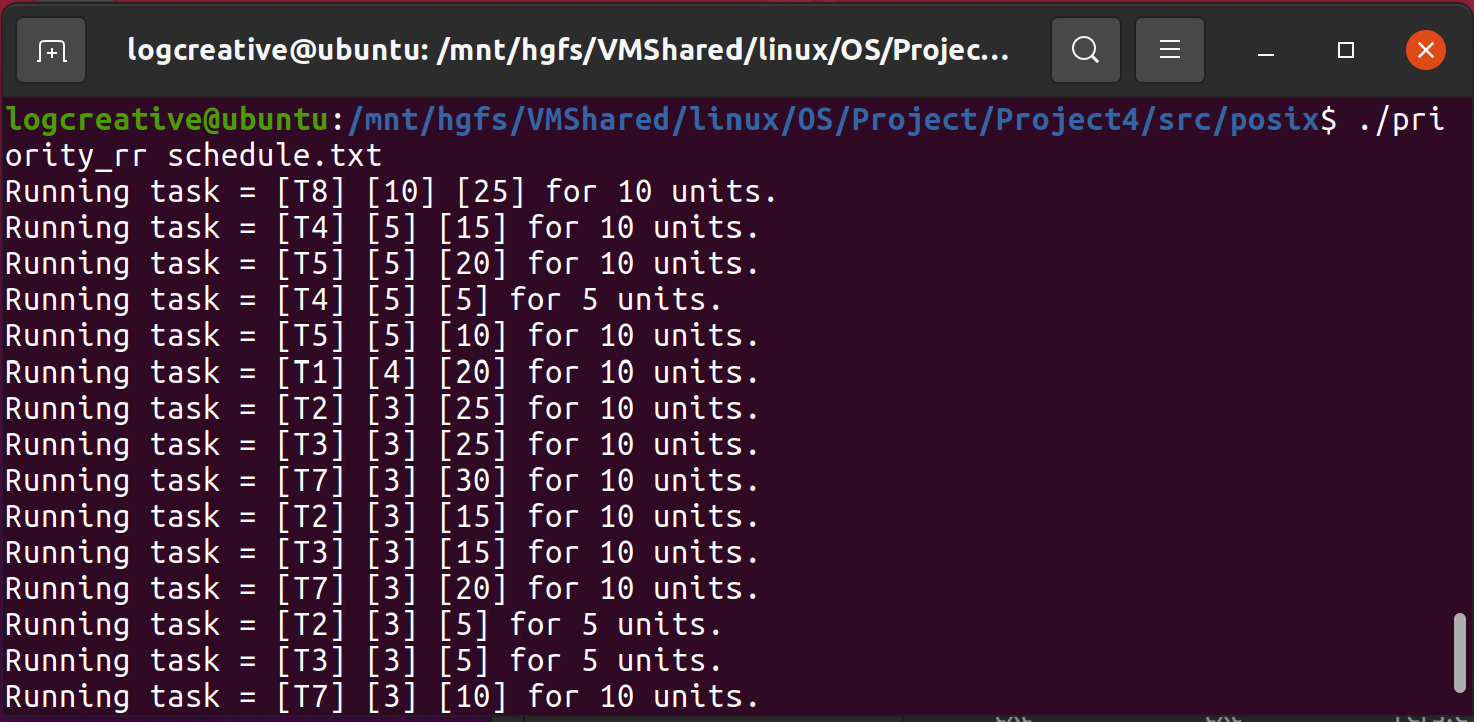
\includegraphics[width=0.8\textwidth]{prrr1.png}

        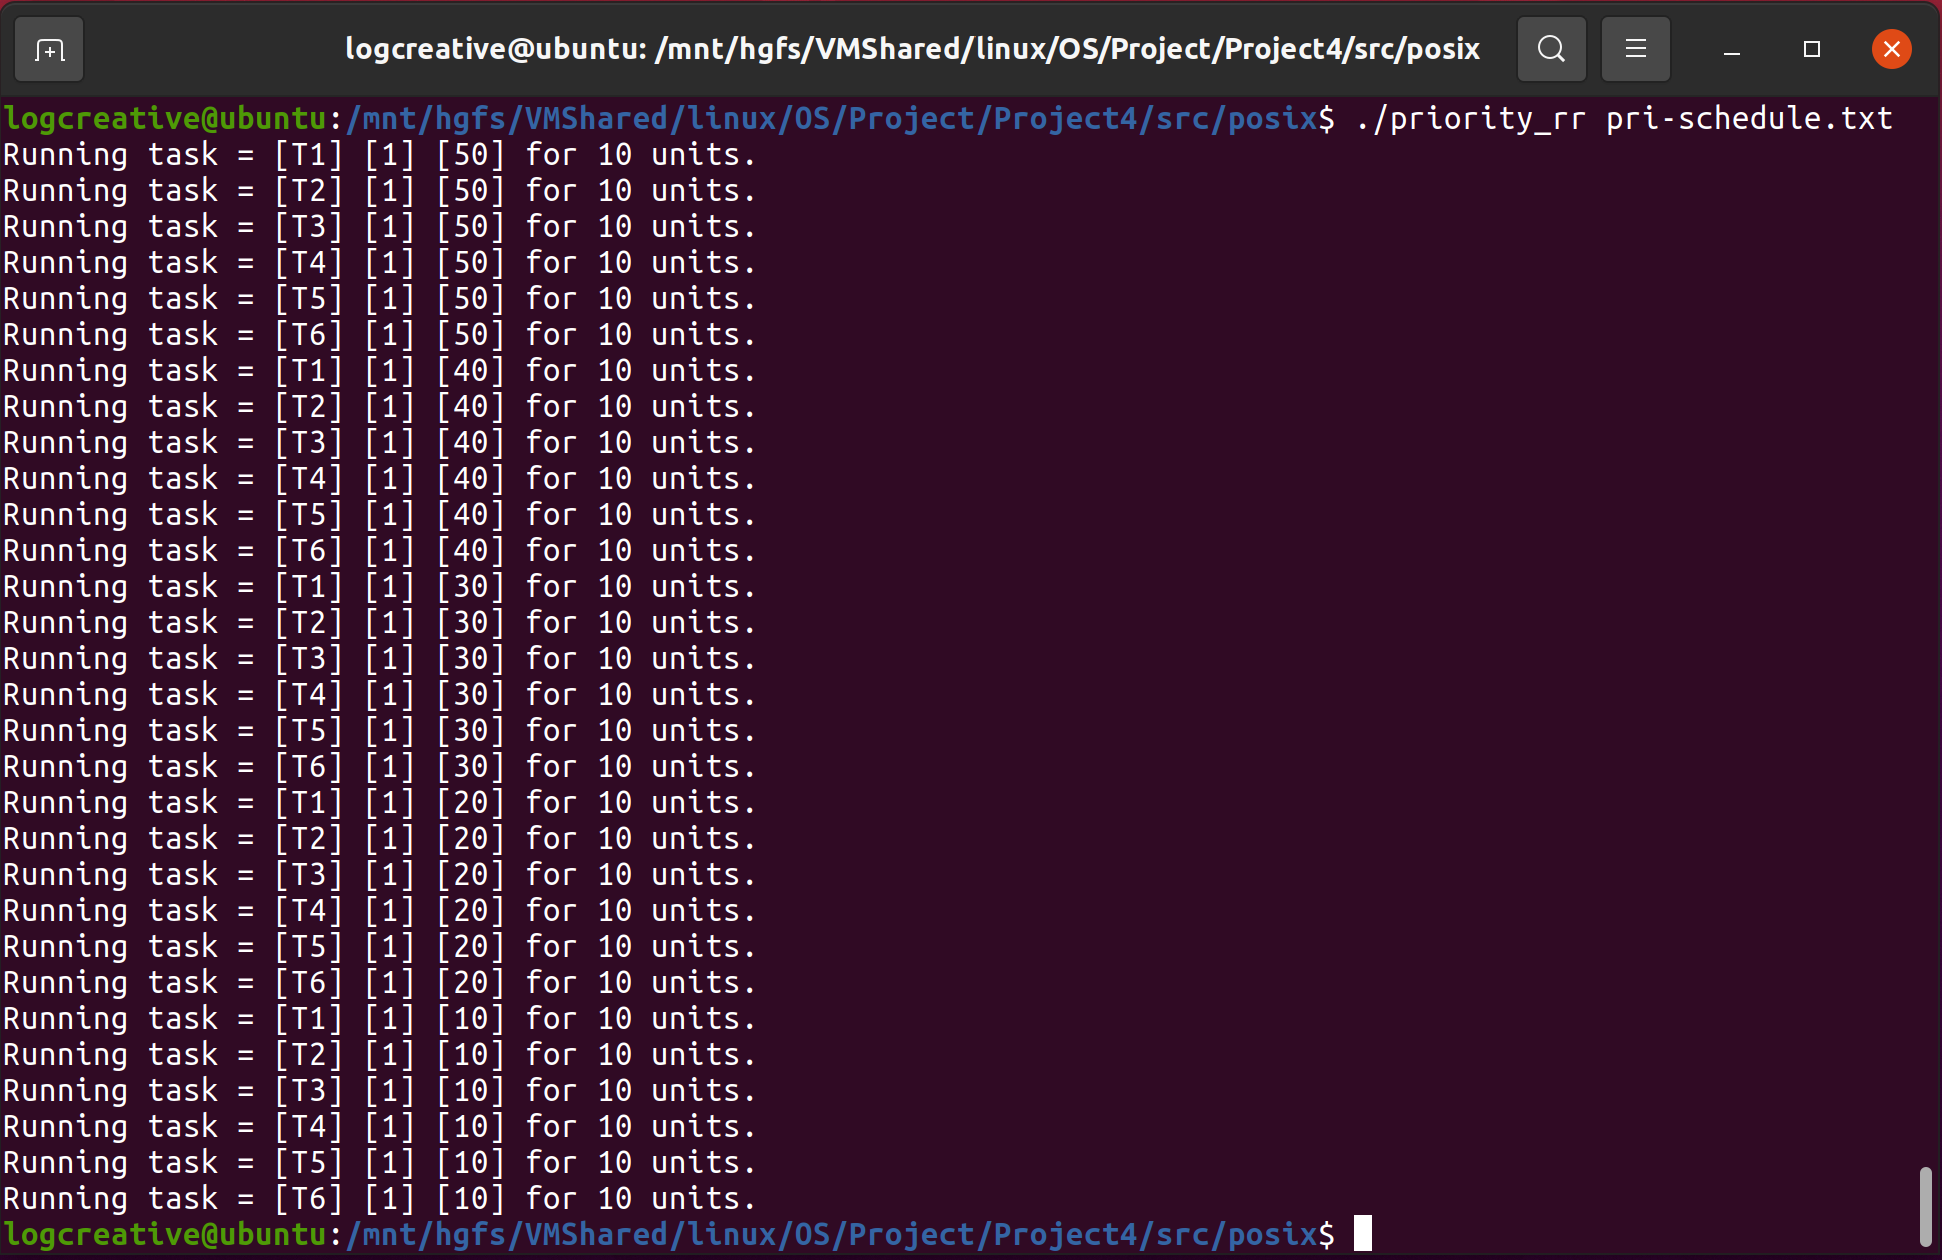
\includegraphics[width=0.8\textwidth]{prrr2.png}

    \end{steps}
    \item[二] 
\end{problems} 

\end{document}
